
\renewcommand\thechapter{\Roman{chapter}}
\chapter{Project context and state of the art}


\newpage
\addcontentsline{toc}{section}{Introduction}
\section*{Introduction}
In This Chapter, we will give an overview of the host organization. Then we introduce cybercrime, hacking, and digital forensics, in the context of our project. Finally we will analyse and compare various existing solutions and present our proposed solution.

\section{Host organization}
\subsection{EY}
EY\cite{ey} is a multinational professional services organization that employs more than 270,000 professionals operating in over 700 offices in 150 countries, which makes its global reach enormous.\\
Some of the services it provides are audit, tax, business risk, technology and security risk services.\\
The objective of EY is to help clients, from start-ups to Fortune 500 companies, identify and capitalize on opportunities.\\
EY is a global leader in its areas of expertise, and is among the top four audit firms that have such a global coverage. These companies are referred to as the "Big Four", including KPMG, PricewaterhouseCoopers (PwC), and Deloitte.\\
The Tunisian experience began in 1987 with the creation of the AMC audit and advisory firm. In 1995, the company AMC became a member of Ernst \& Young's international network, becoming the only representative of the company in Tunisia.\\
To better understand the need and place of forensics in cyber security, we need to talk about cybercrime in general, how an attack happens, and what forensics has to do with it.
\subsection{EY Advanced Cyber Security Team}
EY Advanced Cyber security team is a group of highly qualified security consultants that are able to offer multiple services in cyber security. Below we list the main services that the team can provide:\\
\textbf{Infrastructure Security Assessment} services aim to provide accurate knowledge of the customer's level of security and to provide effective solutions to any weakness in their systems. This category includes traditional services such as ethical hacking, vulnerability assessment in different technology environments (wireless, VoIP, critical networks, Infrastructure) and technical review of IT policy compliance.
\begin{itemize}
    \item Internal Penetration Testing
    \item Wireless Security Assessments
    \item Operational Technology (SCADA) Penetration testing
    \item Smart Grid Penetration Testing
    \item Interactive Voice Response (IVR) System and VOIP security testing
    \item Network and System Infrastructure Configuration Reviews
    \item Virtual Desktop Infrastructure and Citrix Security Testing
    \item External Penetration Testing
\end{itemize}
\textbf{Application Security Solutions} area focuses on the security issues associated with the development of thick, mobile Web applications, poor application design, configuration, and implementation, which continue to be a major contributor to security breaches for organizations. For this, the team has qualified professionals in the field of application security, source code and application architectures.
\begin{itemize}
    \item Web Application and Web Services Testing.
    \item Dynamic Application Security Testing.
    \item Thick Application Testing.
    \item Mobile Application and Device Testing.
    \item Automated and Manual Source Code Review.
    \item Mainframe Infrastructure and Application Testing.
    \item Testing of ATM’s, ATM Switches, Check Processing Machines and POS Device Testing.
    \item Kiosk Testing.
\end{itemize}
\textbf{Red Team} services assess security controls related to defense in depth. They can range from targeted social engineering campaigns to simulated APT attacks. This service is designed to target organizations by prompting or manipulating personnel to provide sensitive information, bypass technical access controls on the network, or to gain unauthorized access to facilities. Red Team conducts these assessments from a variety of attack vectors such as phishing scenarios, USB attacks, specially crafted malware, and physical intrusions, all of which are associated with traditional penetration testing techniques. The goal is to compromise the network without the limitations of a traditional fixed scope like penetration testing.\\
\textbf{Security Training} provides a variety of custom security training courses that enable organizations to quickly, efficiently, and methodically train their personnel and developers to protect their environment and identify vulnerabilities in their information systems. The secure coding classes are designed to provide developers with the skills to develop and manage secure applications. In addition, it provides social engineering and physical security assessments to customers who require a comprehensive assessment of security posture encompassing non-technology assets such as human resources, processes, and organization. This team has successfully applied a risk-based approach to creating, executing, and implementing these types of large programs such as BAU (Business As Usual) audit-mandated, platform upgrade and major versions of high-risk, high-volume projects covering various clients and sectors.

\section{Preliminary study}
\subsection{Cybercrime}
'Cyber crime contains all criminal offences which are committed with the aid of communication devices in a network. this can be for example the Internet, the telephone line or the mobile network' (Wikipedia, 2008).\\
We can conclude that a cybercrime involves the use of digital device to attack another one on a specific network using some types of cyberattacks. The aim of a cyber attack is to steal, corrupt, or hack the information of an individual, an organization, or government office.\\
This is a process used to attempt accessing a system illegally to exploit unauthorized data or other information. This process involves the scanning of the Internet to find systems which could be mis-configured or contain security vulnerabilities. Once a cybercriminal gets access on a system, he can control the infected system and use it to spy on or disrupt services of other systems.\\
Cyber criminals can be anyone you may know or not know, like an annoyed employee, a partner, a competitor, an angry citizen, a terrorist or a bored teenager.

\subsection{Cyber attacks}
We will enumerate some of the most common cyber attacks that are seen daily.
\begin{enumerate}
    \item Phishing\\
    A phishing attack is a method by which an attacker makes himself look trustful so that a target shares his sensitive information thinking it's a legitimate service. These attacks can be seen in a form of an email, a phone call, or a website that tries to look legitimate. The name comes from the fact it's the same as catching fish, a hacker would use a website that looks like Paypal, for example, and lure the target into it so that he sends his personal and sensitive data, including credit card, home address, and phone number. An example overview of this attack type is shown in Figure I.1.
    \begin{figure}[H]
    \centering
    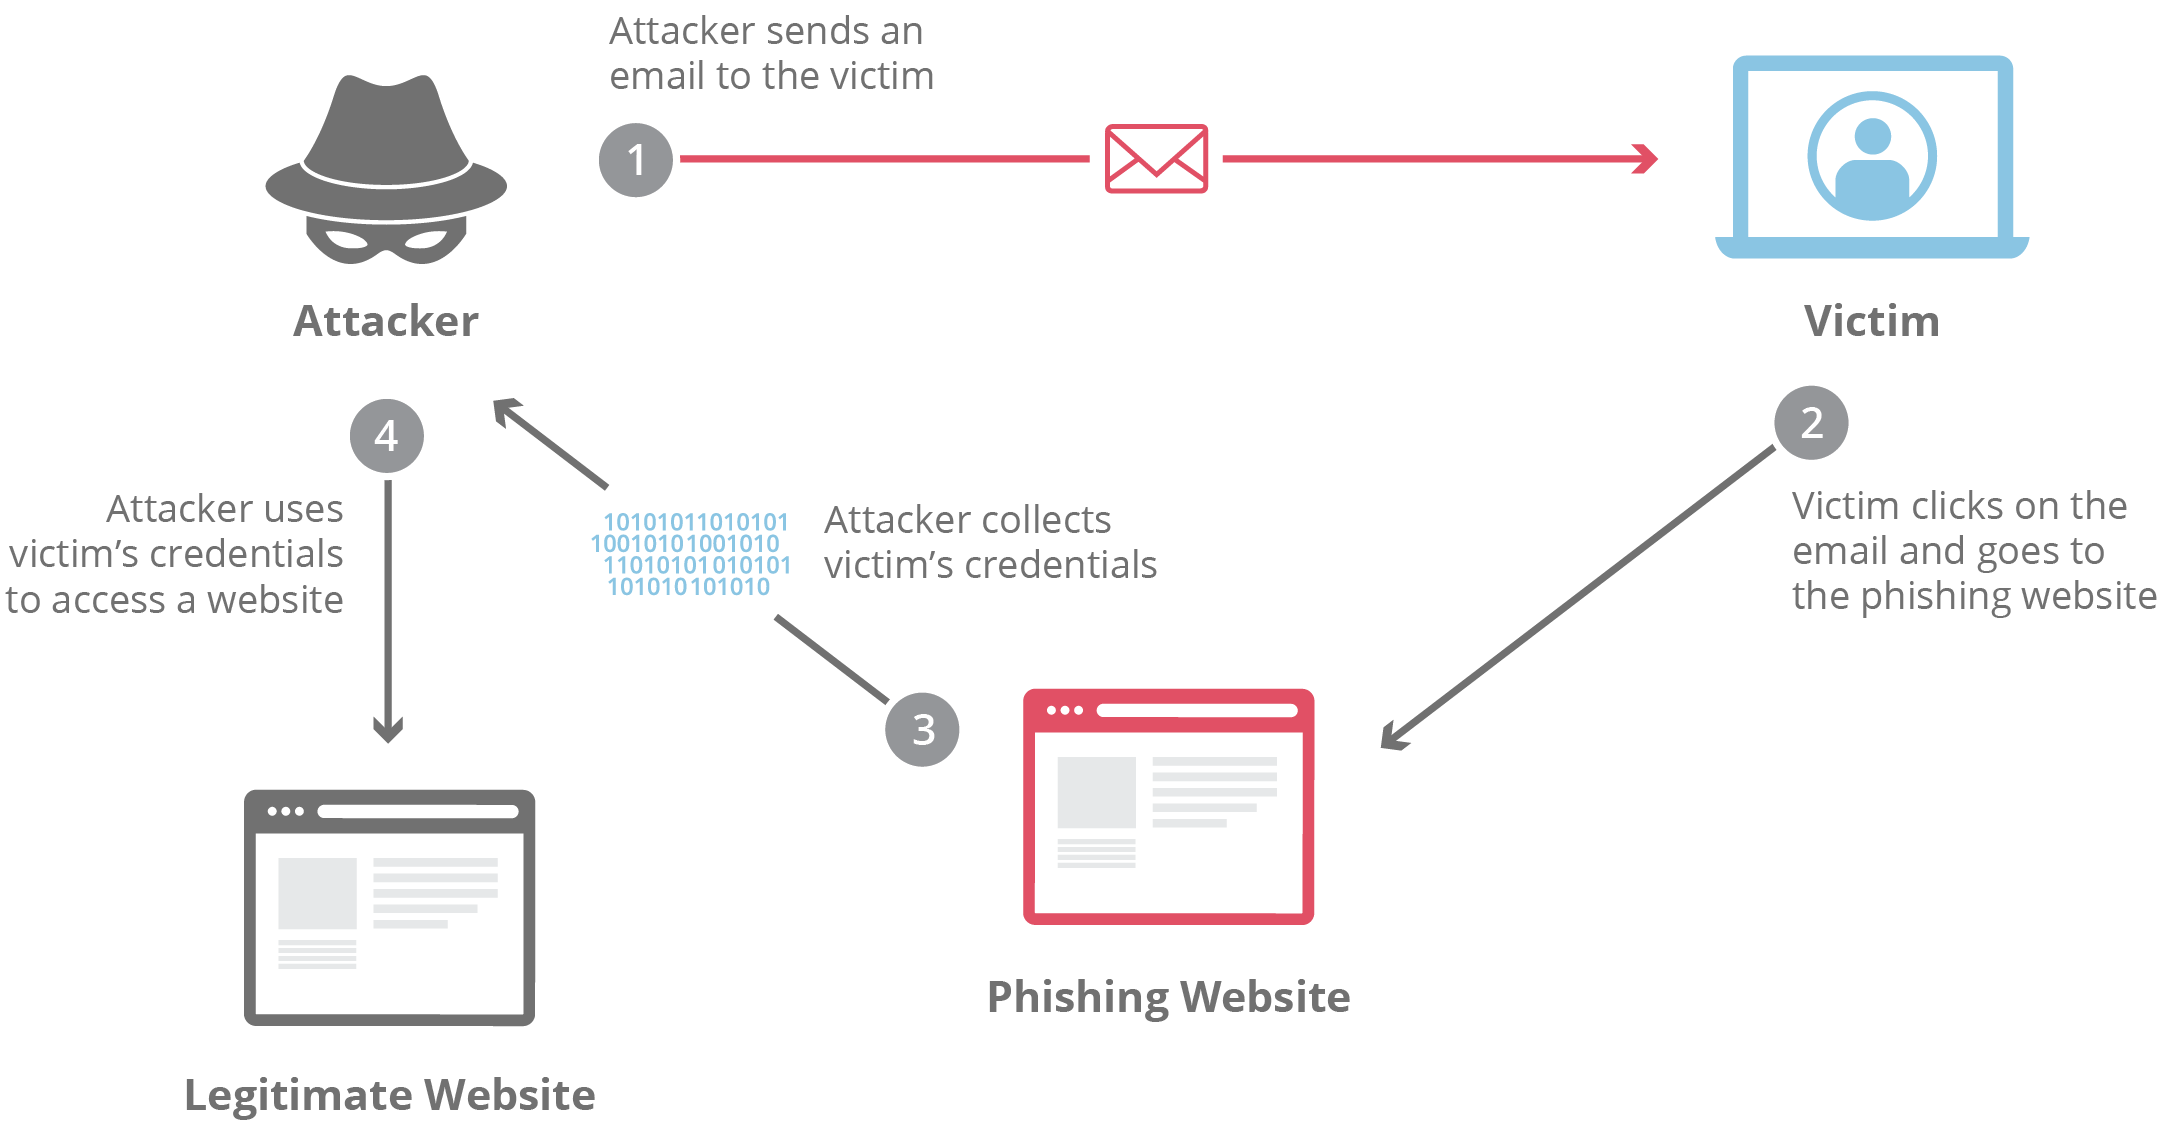
\includegraphics[width=0.7\columnwidth]{Figures/phising.png}
    \caption{Phishing attack \cite{phishing}}
    \end{figure}
    \item MITM\\
    A man in the middle attack is like eavesdropping but in a more advanced way. An attacker would be able to insert himself between two parties when communicating and all the conversation would run by him at first, which can be more understood from Figure I.2. This means that an attacker would actually know what was sent and received without both parties knowing anything about it. The attack can also be used to impersonate one of the parties and send a message from one party to another by signing it as one of them.
    \begin{figure}[H]
    \centering
    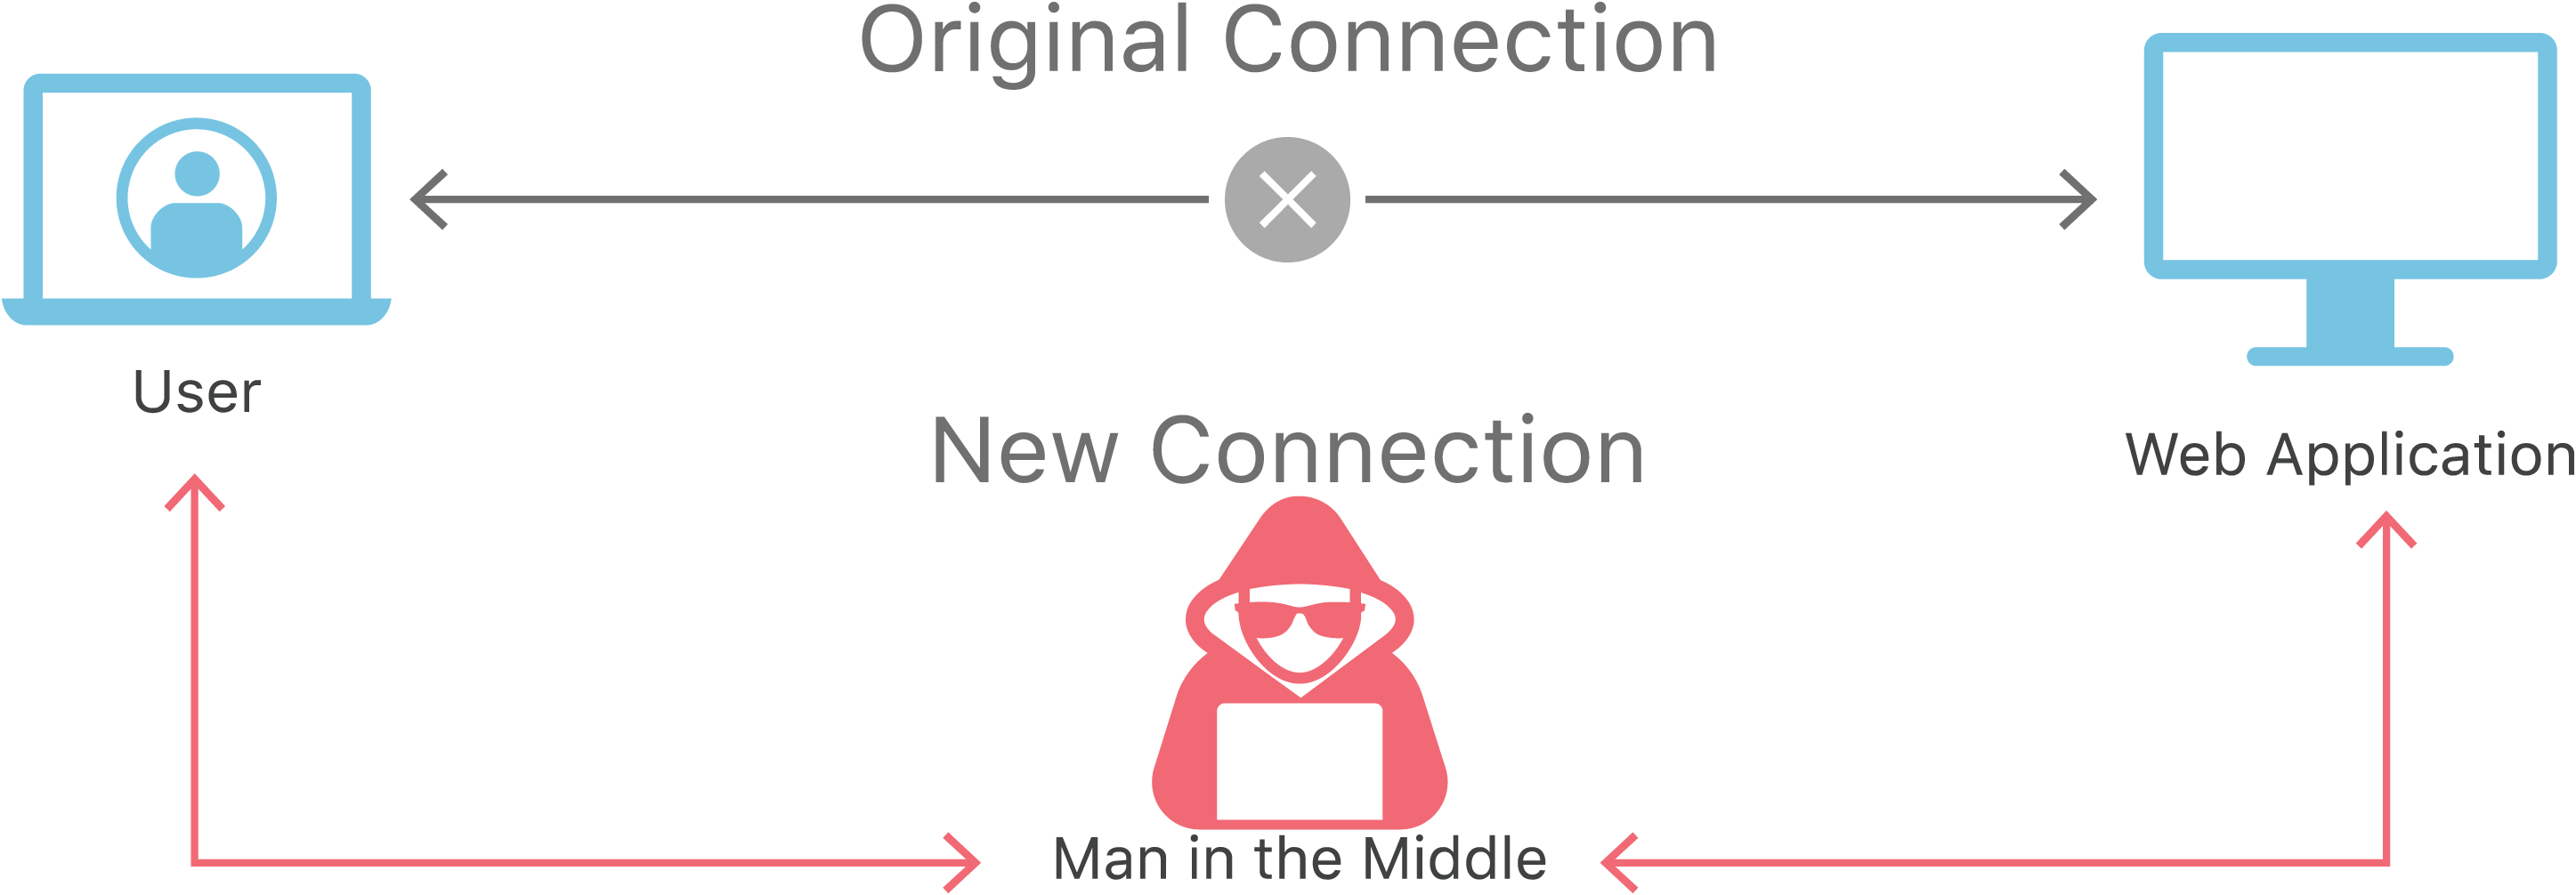
\includegraphics[width=0.7\columnwidth]{Figures/mitm.png}
    \caption{Man in the middle \cite{mitm}}
    \end{figure}
    \item DOS\\
    Denial of service attacks are used on networks and systems to render their services unavailable at a certain time or forever. The impact of such attacks is huge and mostly include economic and productivity losses at high expenses. DOS attacks are sometimes called DDOS (Distributed Denial Of Service), and that's when more than one computer is used in the process (most likely bots), as represented in Figure I.3. An example of how these attacks work can be by flooding the server with a number of requests that exceed the capability of it's buffer and render it unable to reply to normal requests, as follows:
    \begin{figure}[H]
    \centering
    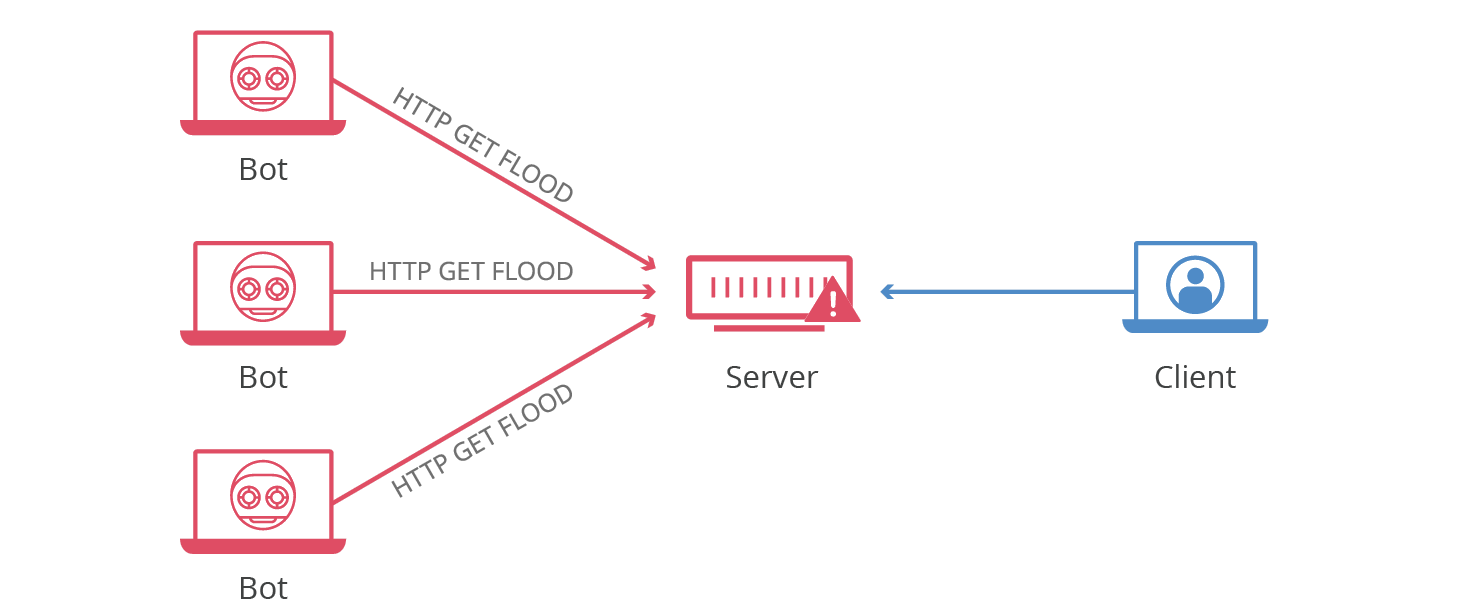
\includegraphics[width=0.8\columnwidth]{Figures/flood_ddos.png}
    \caption{DDOS - HTTP Flood Attack \cite{ddos}}
    \end{figure}
    
    
\end{enumerate}
\subsection{Malware}
A malware is basically any software that is harmful to an electronic device. This can help steal, corrupt, spy, and manipulate data on a computer without the knowledge of the owner.\\
Many types of malware exist. Some are more harmful and malicious than others. Most common type is encountered daily by all internet users, and that is Adware.

\textbf{Adware} are most know for the pop-ups they keep showing on a PC and websites you visit, offering free and exclusive experience like games, websites, and other matters. Figure I.4 shows an overview of what it looks like. It may not look that harmful and people may often leave it after failing to delete it since it doesn't pose a real threat more than a nuisance. But sometimes these software include Spyware or other type of malware that is activated as soon as you click on it.\\
\begin{figure}[H]
\centering
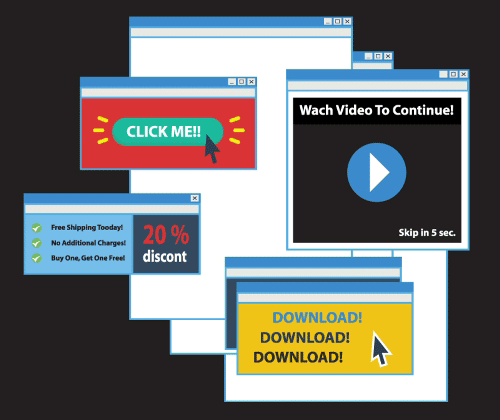
\includegraphics[width=0.5\columnwidth]{Figures/adware.png}
\caption{Adware overview \cite{adware}}
\end{figure}
\textbf{A Spyware} is installed on a host and hidden from the user. It is used to collect data like internet usage, keylogs, passwords, and personal information like we can see in the Hawkeye\cite{hawkeye} screenshot on Figure I.5. It then sends it to the attacker who keeps monitoring your PC this way without your knowledge. Another way to put such malicious software without being detected is integrating it within another legitimate software. In that case it's called a Trojan Horse.\\
\begin{figure}[H]
\centering
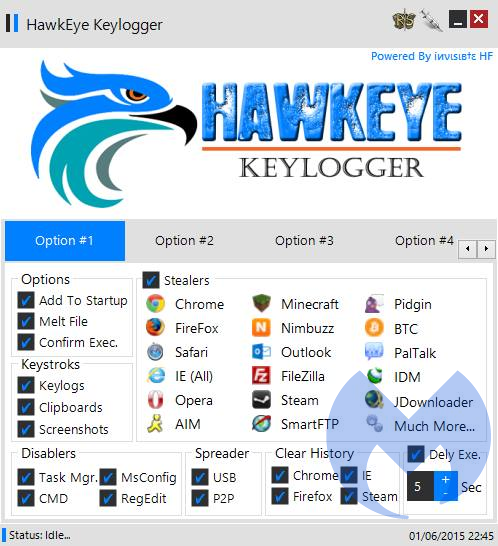
\includegraphics[width=0.6\columnwidth]{Figures/spyware.png}
\caption{Spyware Example \cite{spyware}}
\end{figure}
\textbf{A Trojan horse} is a type of malware that looks legitimate and eludes the user to trust it by pretending to be something the user wants. This software has some malicious code or function inside of it that isn't detected until it's running in the memory. As an example of how it is injected, Figure I.6 represents the Terdot trojan's initial injection chain. In most cases it can't be detected by signature because a good attacker would change variables and function names for each attack, making it have a new signature. While running in the background, a Trojan can install other malware like Ransomware.
\begin{figure}[H]
\centering
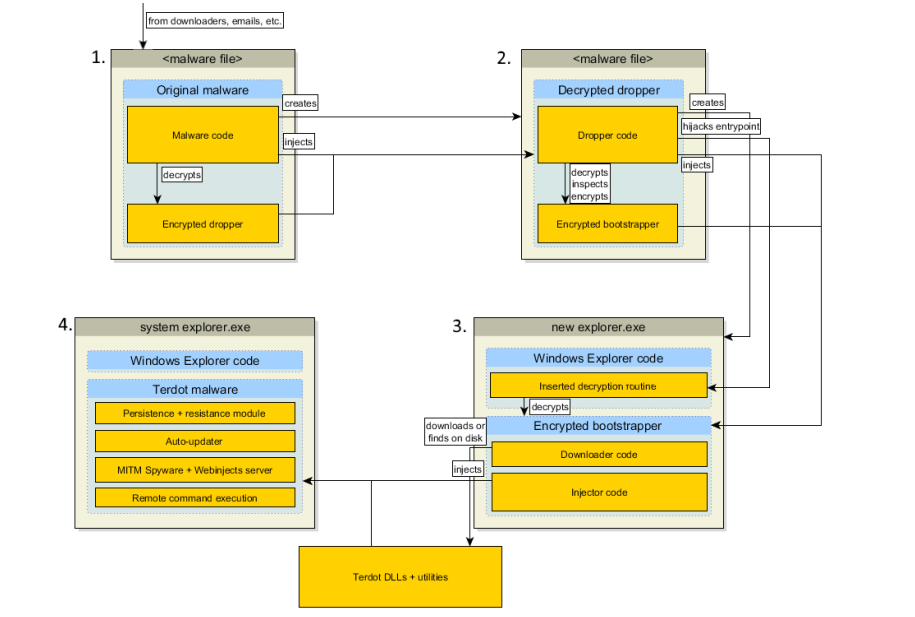
\includegraphics[width=0.6\columnwidth]{Figures/trojan.png}
\caption{Trojan injection process \cite{trojan}}
\end{figure}
\textbf{A Ransomware} is a malicious software that denies access to user's computer or data by encrypting or locking it and threatening to release is to the public or using it in illegal deals. The obvious way to get the data back is only if a ransom is paid to get the decryptor, but it surely doesn't guarantee that the attacker still has your data. The ransom is usually paid anonymously using cryptocurrency like Bitcoin. An example of a ransomware named Wannacry is shown on Figure I.7.
\begin{figure}[H]
\centering
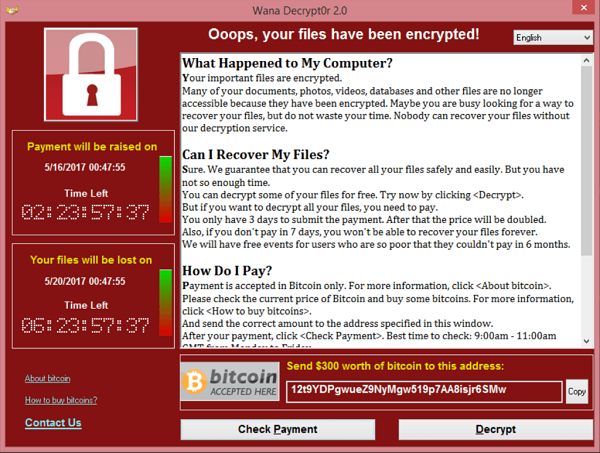
\includegraphics[width=0.7\columnwidth]{Figures/ransomware.png}
\caption{Wannacry ransomware example \cite{ransomware}}
\end{figure}



\subsection{Attack Phases}
There exists many tools that help blue teams to identify, hunt, and track suspicious activity in a network. No matter the steps taken by an attacker, his actions leave a corresponding artifact leaving behind footprints that can be critical. Attacks usually follow a predictable pattern, and we focus our first detection efforts on the set of fixed portions of that pattern.\\
For a better management and securing information systems, one must understand the attacker's view and steps. The phases on Figure I.8 are the 5 general steps a hacker would follow, from selecting his target, to owning the system.
\begin{figure}[H]
\centering
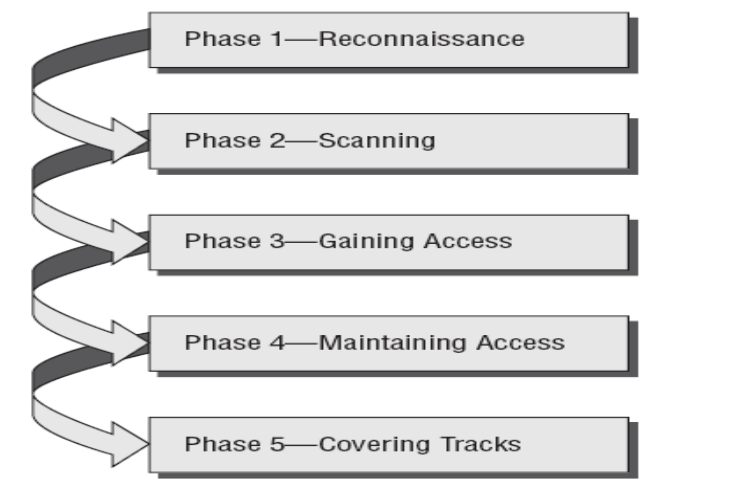
\includegraphics[width=0.6\columnwidth]{Figures/attack_phases.png}
\caption{Cyber Attack Phases\cite{attackphases}}
\label{fig_logo_utm}
\end{figure}
\subsubsection{Reconnaissance}
This phase requires the hacker to collect information about the potential victim. It involves identifying who the target is, and collecting information about it from public records, social media, website, etc. It also involves enumerating any parties involved with the target, like employees, associates, server hosts, previous breaches, etc.
\subsubsection{Scanning}
This phase involves active information gathering. An attacker would try to find out more information about the target by using port scanners, vulnerability scanners, and network scanners to determine any vulnerable data or service that could allow access to the target's machine or network.
\subsubsection{Gaining access}
Based on the collected information from the previous phases, the attacker plans on which attack vector he would go through to potentially have access. Attacks can vary from Social Engineering and Phishing, to exploiting a out-dated service or implementing a 0-day exploit.
\subsubsection{Maintaining access}
After getting access on a user's account in the system, the hacker would need to escalate his privileges to become an administrator and have the right to do anything he would like. The hacker will also need to deploy a backdoor in any form possible so that in case the attack was detected or that user's account got disabled, he would still have access to the network. This could happen by creating a new hidden user or allowing a service through the firewall.
\subsubsection{Clearing tracks}
All is done, The hacker has access and got what he wanted, now it's time to cover the tracks. The attacker will attempt to remove all tracks tracing him back to the attack. This phase is necessary so that no evidence is left for the forensics investigators to find in the system. This would require clearing out temporary files, logs, any data sent over the network, etc.

\section{Red Team}
\subsection{Introduction}
It is not enough to know the steps a hacker follows so we can secure the systems, detect his activities or track him down. The best way to secure your servers is to know it's weak points. Penetration testing allows us to know the vulnerabilities present on our systems and how they can be exploited so that we can take more defensive measures.\\
While Penetration Testing also involves testing for vulnerabilities in a system, network, or application to identify potential entry points for an attacker, it doesn't simulate a real hacking scenario.\\
When conducting a red team assessment, red teamers are required to replicate a real hacking scenario. Only a couple of people in the targeted firm would know about it, and most attack vectors are permitted. Thus, employing a red team assessment challenges a firm's detection and response capabilities effectively, touching most security policies and measures.\\
One of a red team's objectives is to get in without being detected, which involves hiding from defensive measures at first and then pass through the harder part which is not to be tracked down by the forensics investigators.
\subsection{Main Objectives}
\begin{itemize}
    \item Tests the effectiveness of an organization's digital forensics and incident response capability.
    \item Measures the capacity of the organization’s defensive posture.
    \item Provides access to good quality threat intelligence on an organization.
    \item Simulates a more realistic threat environment to the systems.
    \item Qualifies the effectiveness of an organization’s security awareness program.
    \item Ensures a way to build a proactive capability to manage and respond to real threats.
\end{itemize}

\section{Digital forensics}
\subsection{Introduction}
"DF is the scientific study of all the processes, involved in the recovery, preservation, and examination of digital evidence, including audio, imaging and communication devices" \cite{df}

A branch of forensic science that consists of identifying, preserving, recovering, analyzing and presenting facts about digital evidence found on computers or digital storage media devices. So it deals primarily with the recovery and analysis of latent evidence following cybercrimes or a service deficiency.\\
In most cases, an organization would conduct an investigation once a security breach has been detected, but it is essential that organizations take security measures and implement appropriate security policies and monitoring tools, as well as the identification and acquisition of live evidence right away in case of a suspected problem.\\
Computer forensics, or digital forensics in general, can mainly be about but is not limited to legal prosecution activities. A firm would conduct a forensics investigation for various reasons such as intelligence gathering, and finding the root cause of a server-side problem.\\
When being in the circle of attention, it is safe to say that any electronic device you touch will be used against you. Forensics investigations try to gather data from all places to acquire as much and efficient data as needed to prove a point. This is an immense field that is divided into more sub-fields.\\
We will now introduce some of the terms used in Digital Forensics for better clarification of future uses.
\begin{itemize}
    \item Cyber Forensics\\
    Investigative procedures used to collect, examine, analyse, and report findings associated with computing devices and networks, and is made suitable to enter such evidence into the court of law.
    \item Cyber Incident Response\\
    A methodical approach to managing a security breach with the intent of limiting damage, reducing recovery time, reducing costs, and developing a lessons-learned report. The lessons-learned report is used to stop or mitigate the impact of similar events as they occur in the future.
    \item E-evidence\\
    The forensics science involves collecting a set of evidence from a scene. Evidence deriving from any electronic source is called E-evidence.
\end{itemize}

\subsection{E-evidence sources}
E-evidence can be acquired from a lot of different devices. Each device has it's own specifications. We are to be focusing on computer forensics, as such, we shall present where we'll be getting evidence to be analysed later on.
\begin{itemize}
    \item Memory dump\\
    The memory data that sits on the Random Access Memory (RAM), should be retrieved immediately before anything due to the fact that it is volatile and would be lost in case of a system shutdown. This data contains the list of anything that was running or happened when the system was on. This list can include and is not limited to processes, internet browsing history, files accessed, network connection, logged in users and their hashes.
    \item Disk image\\
    Getting data from a non-volatile memory, which can be found on a computer’s hard disk drive, solid state drive, or external drive, would require keeping that drive for the whole investigation process or at least it's content. To keep that content as it is without keeping the hard disk, we need to take an image of it. A disk image is an exact copy of the contents on a hard drive and is stored on another device, and not stored on the hard drive from which the copy was made.
    \item Network traffic\\
    Network traffic is transmitted and then lost, so the analysis of this data is often pro-active, but we can record it using a network sniffer to analyse it at any other time. The traffic contains the list of packets transmitted through the network including connections made with other parties, protocols used, payloads sent and received. We can scan this data to potentially find malicious payloads that could be a cause of an attack or follow the identity of a possible attacker.
\end{itemize}

\subsection{Types of digital forensics}
Digital forensics involves the analysis of various hardware contents, each having it's own specifications. We will list and explain some of the most common types of forensic analysis.
\subsubsection{File system analysis}
File system forensics is the examination of storage devices like hard disks and USB sticks, in order to extract valuable information.\\
A disk contains all user files that could contain a lot of evidence and logs to help us later on in the analysis. We could also recover deleted files, metadata and sessions from different systems.

\subsubsection{Memory analysis}
Memory forensics refer to the analysis of volatile data from a computer which is exported into physical file dump.\\
Since everything that happens on a computer passes through the RAM first, like opened files, programs (processes), and network connections, we need to dump and analyse it in order to understand what happened on the system when it was up.\\
That is why new attacks use techniques that leave no traces on disk but only on live memory since it will be lost later.

\subsubsection{Network analysis}
Intrusion detection systems will play a key role as input data sources for network forensic analysis into the foreseeable future. This is especially true because they are very commonly used methods of capturing data from a wide variety of digital sources and storing that data in a centralized repository that could be made accessible to analytical processes with forensic objectives.\\
Performing network forensic analysis will require critical observance of large amounts of highly filtered data from varying sources, many times over large geographic spaces. This complexity causes concerns in related matters like how often the data or snapshots are to be collected, who is to collect the data, since it needs to be taken immediately, and there needs to be certain level of trust in that party, and what exactly is to be collected and what to filter out.

\subsubsection{Mobile analysis}
Mobile device analysis relates to the recovery of digital evidence or data from a mobile device.\\
An estimated 66.7\% of the population worldwide owns a cellphone by now. This increases the probability that if a certain person is involved in a crime or an anomaly that happened to a system, we would find some data referring to it somewhere in his mobile devices. Although that probability may not be high enough, but it's getting higher since a modern human's mindset would require him to at least plan it on an electronic device.\\
Data recovered from these devices can be pretty helpful. We could recover GPS-saved location history, call logs, contacts, images taken by the user and even the deleted one's.

\subsubsection{Log analysis}
Log analysis is actually one that we talk about the least, but end up doing the most. SIEMs were supposed to keep us from needing to do this, but a good way to understand exactly what happened is to keep reading the logs from the system and software affected. Analyzing log falls into system anomalies detection, in most cases. Since services and implemented monitoring solutions keep track of every action that takes place on a system, it is inevitable to produce a timeline through the logs to understand where something went wrong and follow it to the root cause.

\subsection{Digital forensics models}
Digital forensics is part of a security approach. It can help with the after-incident, but has also evolved to deal with detected attacks or crimes on the go. These approaches are known as Reactive and Proactive forensics.
\subsubsection{Reactive}
This is the traditional or post-mortem approach of investigating a digital crime after an incident has occurred, which we will research more for the purpose of this report. This involves identifying, preserving, collecting, analyzing, and generating the final report. Two types of evidence are gathered under this component:
\begin{itemize}
    \item Active: Active evidence refers to collecting all live (dynamic) evidence that exists after an incident. An example of such evidence is processes running in memory.
    \item Reactive : refers to collecting all the static evidence remaining, such as an image of a hard drive.
\end{itemize}
\subsubsection{Proactive}
Proactive Digital Forensic Component has the ability to proactively collect data, preserve it, detect suspicious events, gather evidence, carry out the analysis and build a case against any questionable activities. In addition, an automated report is generated for later use in the reactive component. The evidence gathered in this component is the proactive evidence that relates to a specific event or incident as it occurs.\\
As opposed to the reactive component, the collection phase in this component comes before preservation since no incident has been identified yet. This approach is also more useful for detecting attacks using Anti-Forensics.


\subsection{Anti-Forensics}
The term anti-forensics refers to methods that prevent forensic tools, investigations, and investigators from achieving their goals. Any methodologies that used to incriminating computer forensic process can be considered as a anti forensic. Basically, there are four types of anti forensic technique such as destruction, evidence source elimination, evidence hiding, and evidence counterfeiting.. From a digital investigation perspective, anti-forensics can do the following:
\begin{itemize}
    \item Prevent detection of digital crime.
    \item Provide misleading evidence that can jeopardize the whole investigation.
    \item Prevent evidence collection.
    \item Obfuscate data that could lead to evidence.
\end{itemize}

\subsection{Stages of digital forensics}
The traditional digital forensics follows the reactive model which consists of 5 stages followed by investigators to conduct the investigation. These stages can be named, described, or grouped otherwise, so we are following the steps of a DF handbook\cite{handbook} as presented in Figure I.9.
\begin{figure}[H]
\centering
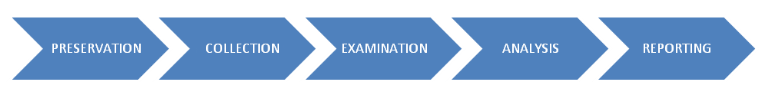
\includegraphics[width=1\columnwidth]{Figures/foren.png}
\caption{Digital forensics process}
\end{figure}
\subsubsection{Preserve}
This is a fundamental element in all digital forensics activities. If potential evidence is not preserved in the correct manner, then it may have little or no value in any criminal or civil proceedings, although it may still be useful for gathering basic information about a case. The preservation of evidence must be conducted by staff that acquire the skills and techniques required and use of the appropriate tools to preserve the evidence in an unaltered state. Developed and tested procedures that are known to be accepted by the courts should be followed whenever possible. The preservation of evidence is most important and must be considered at all stages of the investigation.
\subsubsection{Collect}
The collection of any digital device or information that may be used as evidence must be carried out by trained staff and must follow specific procedures so that its value as evidence is preserved for the analysis and usage in any legal or disciplinary proceedings.
\subsubsection{Examine}
The examination of evidence must be carried out using tools that have been tested or accepted by the courts as providing information in a faithful form. Any data produced for the purposes of proof must be reproducible by another investigator. The examination of the evidence must be thorough and in a comprehensive manner. The examination of the evidence should, as far as possible, focus on an image of the original material rather than on the original material itself, although it is recognized that, in exceptional circumstances, this might not be possible.
\subsubsection{Analyse}
Evidence analysis is the forensic phase in which the information held and examined is interpreted as allowing conclusions to be drawn and the truth about what happened during and before an incident. This will normally be done in the computer forensics lab and care should be taken to ensure that any results are documented and can be recreated by another investigator.
\subsubsection{Present}
The presentation of the results of the analysed data is as important as any other phase of the DF process. If the results are not presented in a coherent, comprehensive and credible form, the efforts made in the previous phases will have been in vain.


\section{Study of the Existing Solutions}
This section presents a study of the most popular existing digital forensics tools. We tried to classify and compare them to each other, and conclude their limits to finally present our proposed solution.
\subsection{Analysis of the Existing Solutions}
DF is one of the most complex science fields. It requires attention and precision in most of it's phases, that following all of them manually would not get the job done. A lot of tools started to appear, each tool simplifies one of the processes and they hardly regroup more than one phase due to the sub-processes in each of them. Most DF tools simplify a set of steps rather than automate a whole process but it's been very useful.
\subsubsection{Description of the most popular solutions}
This section covers a large number of penetration testing tools ranging from free open source software to commercial ones.
\begin{enumerate}
\item \textbf{Volatility} \\ Open-source memory analysis tool which could extract useful data like processes and network connections from memory dumps. Volatility is widely used when analyzing memory dumps, but requires an experienced investigator to know the plugins to be used and regroup the acquired data to then analyse it efficiently.
\item \textbf{Rekall} \\ An open-source memory analysis tool that was historically a fork of the Volatility memory analysis framework and is now more advanced, that it comes with a complete platform for acquisition and analysis.
\item \textbf{Encase} \\ A software that allows the investigator to conduct in depth analysis of user files to collect evidence from a seized hard drive such as documents, internet history and Windows Registry information. Encase is a professional software that can be really expensive depending on which product is needed.
\item \textbf{FTK} \\ Software package developed by AccessData. It enables the acquisition, analysis and extraction of multiple data from a computer disk, such as deleted files and text search. The set of tools in FTK are handful when acquiring dumps of live memory or hard disk, and getting information out of it.
\item \textbf{NIKSUN NetDetector} \\ 
A full-featured appliance for network security surveillance, anomaly detection, and forensics. It complements existing network security tools, such as firewalls, IDS, and IPS. NetDetector should be installed before-hand to detect threats and log connections. The price for NetDetector is rather high but is relevant for the tasks it accomplishes when used correctly.
\item \textbf{NetworkMiner} \\ 
A network analysis tool developed for windows which is available in free and professional edition. It is used to analyse network traffic and allow regenerating files and data transmitted through that traffic.
\end{enumerate}
\subsubsection{Comparison between the studied solutions}
Each one of the tools mentioned specifies in a certain category. But we will try to compare them based on the phases and options they can provide. 
 Table \ref{tab_val} presents a comparison between the existing Penetration testing platforms.
\begin{hyphenrules}{nohyphenation}
\begin{table}[H]
\caption{Comparison between the studied solutions}
\centering
\begin{tabular}{|>{\columncolor[gray]{0.9}}p{2.5cm}|p{2cm}|p{1.8cm}|p{1.8cm}|p{1.8cm}|p{2.3cm}|p{2.3cm}|}
\hline
\textbf{} & \cellcolor[gray]{0.9}\textbf{Volatility} & \cellcolor[gray]{0.9}\textbf{Rekall} & \cellcolor[gray]{0.9}\textbf{EnCase} & \cellcolor[gray]{0.9}\textbf{FTK} & \cellcolor[gray]{0.9}\textbf{Net Detector} & \cellcolor[gray]{0.9}\textbf{Network Miner} \\ 
\hline 
Memory Forensics & \cellcolor{green!25}YES & \cellcolor{green!25}YES & \cellcolor{green!25}YES & \cellcolor{red!25}NO & \cellcolor{red!25}NO & \cellcolor{red!25}NO \\ 
\hline
Disk Forensics & \cellcolor{red!25}NO & \cellcolor{red!25}NO & \cellcolor{green!25}YES & \cellcolor{green!25}YES & \cellcolor{red!25}NO & \cellcolor{red!25}NO \\ 
\hline
Network Forensics & \cellcolor{red!25}NO & \cellcolor{red!25}NO & \cellcolor{red!25}NO & \cellcolor{red!25}NO & \cellcolor{green!25}YES & \cellcolor{green!25}YES \\ 
\hline
\hline
Acquisition & \cellcolor{red!25}NO & \cellcolor{red!25}NO & \cellcolor{green!25}YES & \cellcolor{green!25}YES & \cellcolor{green!25}YES & \cellcolor{red!25}YES \\
\hline
Analysis & \cellcolor{green!25}YES & \cellcolor{green!25}YES & \cellcolor{green!25}YES & \cellcolor{green!25}YES & \cellcolor{green!25}YES & \cellcolor{green!25}YES \\ 
\hline
Reporting & \cellcolor{red!25}NO & \cellcolor{red!25}NO & \cellcolor{red!25}NO & \cellcolor{green!25}YES & \cellcolor{red!25}NO & \cellcolor{red!25}NO \\
\hline
Cross-platform & \cellcolor{green!25}YES & \cellcolor{green!25}YES & \cellcolor{green!25}YES & \cellcolor{red!25}NO & \cellcolor{green!25}YES & \cellcolor{red!25}NO \\ 
\hline
Swap analysis & \cellcolor{green!25}YES & \cellcolor{green!25}YES & \cellcolor{red!25}NO & \cellcolor{red!25}NO & \cellcolor{red!25}NO & \cellcolor{red!25}NO \\ 
\hline
\end{tabular}  
\label{tab_val}
\end{table}
\end{hyphenrules}
\subsubsection{Limits of the Existing solutions}
Conducting a digital forensics investigation requires expertise in the attack and defense fields and expertise in the forensics science, which would be hard and boring, at some point, without automating some of the steps included in these investigations. That is why some organizations opt to buy highly expensive software that can do some of the work in one of the different investigation phases, but not all of them.\\
The reality is that no one tool does it all. Most software touch only one category and no more than two phases, and are also sold with a very high expense. As a consequence, budget permitting, labs need to have a variety of tools available. These software can bring some capabilities to the table, that general-purpose tools don't offer, but should be used mostly in law enforcement forensics labs.\\
All of this led to our solution that supports and combines different forensic analysis types while including some open-source tools and extracting data in all at once using these tools automatically, which we will get to in the next section.

\subsection{Proposed Solution}
Using a lot of tools that require a lot of dependencies and handling can be tiring, especially the first couple of steps when extracting and visualizing acquired data before proceeding to analysis and detection of problems or anomalies, finding a culprit, or following and understanding the footsteps of an attacker.\\
The consultant will be required to acquire digital evidence, and extract the most out of it, leading to an explanation of what happened, how it happened, and why it happened.\\
Like any other process in the information security field, it needs intelligence, observance and concentration to reverse engineer an attack. Following that, automated digital forensics has received a lot of criticism from professionals for that it can't detect a large variety of vectors even when considering dynamic forensics using artificial intelligence. However, critics also currently accept a certain level of automation to help them in their daily tasks.
Manually extracting processes and files and comparing them and scanning each one alone is impractical. We can confirm that automating certain phases in computer forensics would assure:
\begin{itemize}
    \item  Increasing productivity by reducing the time taken to perform repetitive tasks.
    \item  Ensuring that main tasks will run effortlessly and the same way every time it is run.
    \item  A seamless platform integrating your needs.
\end{itemize}
In order to achieve our objectives, we propose to develop a platform that consolidates most useful computer forensics tools and can automate the regroup, summarizing of useful extracted data, and automatic identification of issues given a certain evidence file, which could be a memory dump, network flow, or disk image. This will allow to react better, more intelligently, and possibly fix your next step in the analysis.\\
Some of the function the platform will take care of are these:
\begin{itemize}
    \item Extraction of processes and running them through YARA rules, from memory dumps.
    \item Listing Internet activity, files, GUI, from memory dumps.
    \item Extraction of logs, deleted files, and media, from disk images.
    \item Summarizing network connections and extraction of files in network traffic.
    \item Detection of common suspicious activities.
    \item Detection of malware, keyloggers, and suspicious connection.
\end{itemize}
Our solution also focuses on fixing two problems in today's digital forensics tools:
\begin{itemize}
    \item They were designed to help investigators find specific pieces of evidence, not to assist them in investigations.
    \item They were designed to solve crimes against people where the evidence is digital, not to assist in solving crimes committed with or against computers.
\end{itemize}
\addcontentsline{toc}{section}{Conclusion}
\section*{Conclusion}
Throughout this chapter, we introduced the host organization in which the project was developed and maintained. We then presented a theoretical research on cybercrime and digital forensics. We have also mentioned and compared some of the different solution used by digital forensics investigators. Finally, we introduced our solution and project objective. This chapter allows us to understand the needs and limitations that we need to overcome, which will lead to understanding the platform's requirements that we will analysis in the next chapter.